% EDITED 2026-09-15 scripts/patch_value_continuum_declared_cencov_2026-09-15T1540.py
% EDITED 2026-09-15 scripts/patch_reversible_continuity_fossil_2026-09-15T1525.py
% EDITED 2026-09-15 scripts/patch_supertask_refs_2026-09-15T1000.py
% EDITED 2026-09-12 scripts/patch_aaronson_chapter_cite_2026-09-12T1300.py
% EDITED 2026-09-11 scripts/patch_splice_jaynes_insert_2026-09-11T1130.py
% EDITED 2026-09-10 scripts/patch_quoting_and_typography_2026-09-10T0620.py
% EDITED 2026-09-09 scripts/patch_duplicate_citekeys_2026-09-09T1630.py
\section{What is a quantum state?}
\label{sec:what_is_a_quantum_state}
We begin at the beginning and work step by step towards deducing some free parameters of the
Standard Model.
\subsection{The problem}
We first need to understand what a quantum state actually represents. After 100 years of quantum
mechanics there is still no agreement. The clearest and most succinct comment on the subject is
from E.T. Jaynes \autocite{Jaynes_89_a}
\begin{quotation}
Because this position seems to arouse fierce controversy, let me stress our motivation: if
quantum theory were not successful pragmatically, we would have no interest in its
interpretation. It is precisely because of the enormous success of the QM mathematical formalism
that it becomes crucially important to learn what that mathematics means. To find a rational
physical interpretation of the QM formalism ought to be considered the top priority research
problem of theoretical physics; until this is accomplished, all other theoretical results can
only be provisional and temporary.
\end{quotation}
In the same article he followed it up with ;-
\begin{quotation}
But our present QM formalism is not purely epistemological; it is a peculiar mixture describing
in part realities of Nature and in part incomplete human information about Nature all scrambled
up by Heisenberg and Bohr into an omelet that nobody has seen how to unscramble. Yet we think
that the unscrambling is a prerequisite for any further advance in basic physical theory. For,
if we cannot separate the subjective and objective aspects of the formalism, we cannot know what
we are talking about; it is just that simple.
\end{quotation}
So, the first task is to unscramble the quantum omelet so that we know what we are talking
about. We have some pretty good clues to work with. The first and most obvious is that by virtue
of superposition of alternatives, which is uniquely quantum phenomenon a quantum state can
represent the classically inadmissible states which occur in self-referential systems, such as a
computer halting and not halting at the same time \autocite{szangolies_2020} or a statement
being true and false at the same time. This is surely a clue that a quantum state is a
representation of some sort of self-referential thing. In addition if we look at the
\enquote{quantum omelet}, the density matrix, we notice that we can move smoothly between an
entirely mixed state which is a classical probability, and therefore due to some deficit of
knowledge on the part of an agent, it's and epistemological probability, and a quantum pure
state where indeterminacy is understood to be an innate feature of nature, not due to a deficit
of knowledge on the part of an agent and therefore ontological as clearly explained in
\autocite{bruknerzeilinger2001shannon}. This strange state of affairs can be seen clearly in a
Bloch ball where the center of the ball is a completely mixed state, and the surface is a pure
state. Yet the different points of view describe the same physical situation and the shift
between them is entirely dependent on an observer's change in their state of knowledge. Taken
together this suggests we should be thinking in terms of a self-referential state of knowledge.

But to suggest that our inability to predict the moment a radioactive nucleus decays is due to
our own ignorance seems crazy. And yet, the quantum Zeno effect
(\autocite{georgesu_2022, saverio_2013, Misra1977TheTheory}) where a quantum state is prevented
from decay into another state by continually checking to see if it has decayed or not, which is
continually updating an observer's state of knowledge, hints that maybe the observer's state of
knowledge is not entirely disconnected from an apparently ontological state of nature.


\subsection{Self-reference, a universal principle in quantum mechanics}

Self-reference and non-Turing computability exist in many disguises. The most basic forms are
the Liar Paradox, \enquote{This sentence is false} or Russell's Paradox
\enquote{The set of all sets that do not contain themselves}. Lawvere \autocite{Lawvere_1969}
and Yanofsky \autocite{Yanofsky2003} have shown that these all share a common form. These
self-referential loops can also be represented as closed time like loops \enquote{CTCs}, e.g.
the Grandfather Paradox where someone gets into a time machine and goes back in time to kill
their grandfather so that they were never born in the first place to get into the time machine.
From the outside we'd see flickering between existing and not existing, with infinite frequency.
This leads us to another form of non-computablility, the super-task, the first example given by
Thomson's Lamp \autocite{Svozil2009}, where we have a lamp that toggles between being on or off,
suppose it starts out switched on, after the first minute we toggle if off, then half a minute
later we toggle in on, then 15 seconds later we toggle it off, and so on. After 2 minutes we
will have toggled it on and off an infinite number of times. We would have performed an infinite
number of actions. The final state cannot be represented as either on or off but has a perfectly
valid representation as being in a superposition of being on and off at the same time. Also
super-tasks can exceed the bounds of a Turing machine
\autocite{shagrirSupertasksAcceleratingTuring2004,Hamkins_2002,Copeland_2002}. Once we know the basic forms of
self-reference it's easy to see how they're smuggled in to different interpretations of quantum
mechanics.

Self-reference is important in quantum interpretations because all interpretations and toy
models must at some point find a way to accommodate $\ket{TRUE} + \ket{FALSE}$. The idea is the
secret underground connection that unites seemingly quite different views of quantum mechanics.
Usually, the authors of interpretation X introduce self-reference without realizing it or
acknowledging it. It pops up in different disguises. In the Many Worlds Interpretation it takes
the form of the Axoim of Choice, which implicitly draws in an imagined supertask to complete an
infinite number of choices in a finite interval of time (refs), in the retro-causal
interpretation it takes the form of imagined closed timelike loops, and in the Bohmian
interpretation it takes the form of non-locality. Penrose is one of the few authors who
deliberately introduce non-computability into their framework. All interpretations of quantum
mechanics are trying to impose a causal, computable narrative onto an underlying acausal,
non-computable reality, and there's always a bit that doesn't fit. Frauchiger and
Renner~\autocite{Frauchiger_2018} proved that all interpretations of quantum mechanics are
inconsistent in some way. Which is obvious because you can't fit an underlying acausal,
non-computable Nature into a causal, computable framework without having an inconsistency
somewhere. Just like nailing down a carpet that's too big for a room, there will always be bump
left over, all interpretations of Quantum Mechanics are an attempt to nail down an essentially
non-computable carpet to fit inside the bounds of computability, it won't fit, there's alway a
bump left over.
\begin{figure}[H]
  \centering
  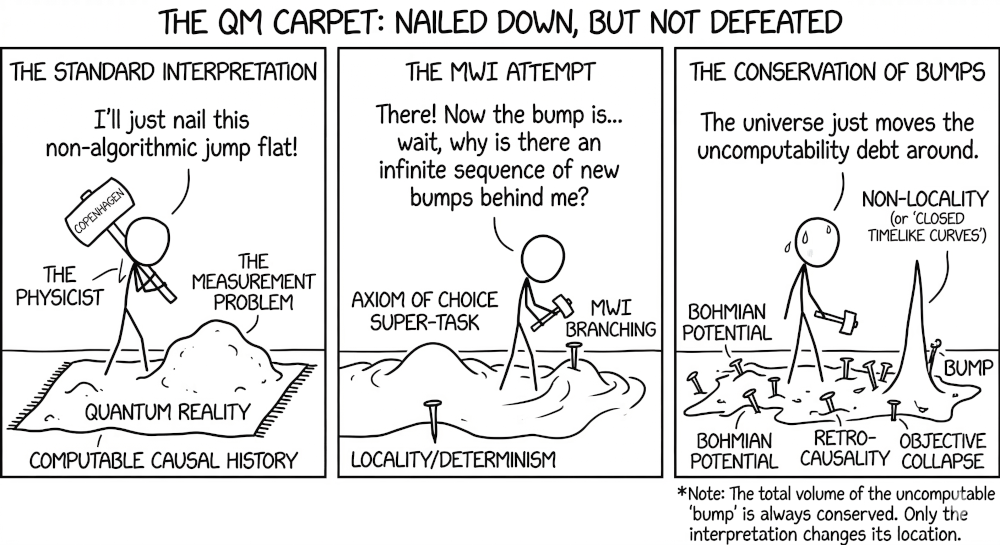
\includegraphics[width=0.85\linewidth]{Gemini_Generated_Image_scaled.png}
  \caption{There's always an inconsistency somewhere}
  \label{fig:myimage}
\end{figure}
The fact that Quantum Mechanics cannot be nailed down to fit our notions of computability is not
a bug, it's a feature we can make use of. Recognising that non-computabilty in its various
disguises has to be smuggled in to any interpretation or toy model of quantum theory relieves us
of the burden of trying to find \enquote{The One True Interpretation}, there isn't one. Instead
we can focus on the more modest goal of finding useful interpretations we can do calculations
with.

Each interpretation of quantum mechanics has its value in understanding some particular facet of
nature, but we shouldn't restrict our affections to just one interpretation. In the same way we
freely switch between different coordinate systems, cartesian, spherical or cylindrical
according to the task at hand we are free to switch between different interpretations according
to the task at hand. We can even switch between entirely different philosophical narrative
coordinate systems as we please. We can be epistemologists in the morning, ontologists in the
afternoon, and followers of the Many Worlds Interpretation in the evening after few beers. Each
has its place and each reveals something useful.

We should take the advice of the great philosopher Groucho Marx~\autocite{marx_1933}
\begin{quotation}
Those are my principles, and if you don't like them... well, I have others.
\end{quotation}
And the same sentiment, but with greater erudition from Edward Gibbon~\autocite{gibbon_1776}
\begin{quotation}
The various modes of worship which prevailed in the Roman world were all considered by the
people as equally true; by the philosopher as equally false; and by the magistrate as equally
useful.
\end{quotation}
We will take the magistrate's view. Is it useful? I'll define "useful" to mean "can we calculate
quantities that can be compared with experiment". It would be extremely boring we resolved
foundational issues in quantum mechanics and it didn't lead to new results. To focus on utility
without affection for any philosophy, then throughout this paper I will freely switch between
different interpretations as is useful for the problem at hand.

\subsection{Karl Popper nails it}
\label{sec:popper}
Returning to the task set by Jaynes, to unscramble the quantum omelet, and here we have a
foundational thought experiment from 1950 by Karl Popper to guide us,
\autocite{Popper1950a, Popper1950b}. It is worth looking closely at what he proposed because it
contains all the essential elements required to understand why we use complex probability
amplitudes in quantum mechanics, and why they have an epistemological origin. In a terrible
irony, having laid the foundations to develop a rationale for an epistemological origin of
quantum probability amplitudes, Popper then spent the rest of his life arguing against any
epistemological view of the matter and developing a propensity view of probability. I
should make it clear that in his 1950 papers he didn't set out to derive quantum mechanics, the
purpose was to show that non-determinism exists even in classical mechanics if we introduce self
reference. It just so happens that his exposition is so clear that he has inadvertently
described nearly everything we need to deduce not just quantum mechanics, but also the Standard
Model.

Because the paper was written before electronic computers were a commonplace fact of life and he
has to describe a mechanical computer which is endowed with the ability to perform all kinds of
calculations, a Universal Turing Machine. Popper speaks about the machine's inability to predict
the outcome of its interaction with its \enquote{closest environment}. I'll change that to say
some entity $E$. We feed into it all the information it needs to calculate the future trajectory
of $E$, and then get the machine to calculate the result of an interaction between itself and
$E$. It can't do it. He writes;-
\begin{quotation}
It is usual asserted (I think correctly) that the physical processes involved in observation
lead to difficulties only in quantum physics and that they disappear if it is assumed that
Plank's quantum of action equals zero - in other words, classical physics. Nevertheless, I
contend that if, in a similar way, we analyze besides the physical processes involved in
observation certain other physical processes which are involved in every prediction, then we
find a somewhat similar result which, however, is valid for classical physics also. The
processes which our analysis must take into account besides observation are the physical
processes involved in the calculation and formulation of the predictions. If this is done then
we find that all scientific predictions are in an important sense deficient, including the most
complete set of predictions possible to formulate even from classical physics; and we find that
this deficiency becomes significant whenever we wish to predict the behaviour of physical
systems (classical or otherwise) of a certain kind, viz, predicting machines.

Our procedure will be to consider some of the properties, and especially the limitations, of
what we shall call the \enquote{predictor}, i.e. a classical mechanical calculating and
predicting machine which is so constructed as to produce permanent records of some kind (such as
a tape with holes punched in it) capable of being interpreted as predictions of the positions,
velocities, and masses of physical particles. It will be shown that such a machine can never
fully predict every one of its own future states and consequently not those of what we shall
call its (closer) \enquote{environment}, i.e. the part of the world with which it (strongly)
interacts. Such a machine, moreover, can never fully predict, or be predicted by, any
sufficiently similar machine with which it interacts. ...
  \par
\hfill \autocite[p.~118]{Popper1950a}
\end{quotation}
\par
He describes a classical mechanically operating \enquote{predictor} $C$ which is set the task of
predicting the result of interaction with its closest environment, we might say the result of a
future interaction with one element of its environment $E$ about which it has been programmed
with complete information. Here it is appropriate to use the epistemological view of probability
as expressed by T. Jaynes because the predictor is attempting to calculate the outcome of a
future interaction between itself $C$ and an external entity $E$ and that prediction is a state
of belief encoded in the physical components of the predictor. We might consider the predictor
$C$ to be a very visibly classical mechanism, such as a Babbage-Lovelace Analytical Engine
\autocite{Menabrea1843SketchBabbage}. Popper then writes;-
\begin{quotation}
Now if it is impossible for $C$ completely to predict its state (i.e. that of its tape) for
\emph{any} moment of its future, we may have to conclude that it will also be impossible for it
to predict completely the state of its closest environment.
  \par
\hfill \autocite[p.~178]{Popper1950b}
\end{quotation}
\par
Replacing \enquote{its closest environment} with $E$ for \enquote{External Entity} we can see
that because $C$ cannot predict its own future state then it cannot predict the outcome of an
interaction with $E$, i.e. a measurement of $E$. But since the outcome of a measurement is
co-determined by $E$ and $C$ together, then $C$ can just as well calculate a probability for the
outcome of the measurement by assuming that it does have perfect knowledge of its own state at
the moment of interaction and that the indeterminate result of a future measurement is a
consequence of some innate feature of $E$ alone. Something Jaynes calls
\enquote{the mind projection fallacy}
\begin{quotation}
It is very difficult to get this point across to those who think that in doing probability
calculations their equations are describing the real world. But that is claiming something that
one could never know to be true; we call it the Mind Projection Fallacy. The analogy is to a
movie projector, whereby things that exist only as marks on a tiny strip of film appear to be
real objects moving across a large screen. Similarly, we are all under an ego driven temptation
to project our private thoughts out onto the real world, by supposing that the creations of
one's own imagination are real properties of Nature, or that one's own ignorance signals some
kind of indecision on the part of Nature. \hfill \autocite{Jaynes1989}
\end{quotation}

Popper then goes on to introduce another predictor $C^+$, which has the same mechanisms as $C$.
This new predictor, $C^+$ is provided with the initial state of $E$ and $C$ and proceeds to
calculate the future motions of all the components. From the point of view of $C^+$ the
interaction between $E$ and $C$ is completely deterministic, there is no sudden jump in state
when $C$ interacts with $E$. $C^+$ succeeds in calculating the outcome of the interaction
between $E$ and $C$ with perfect accuracy, and calculates that after the interaction $C$ and $E$
are correlated. But it would find that it can't calculate an outcome of its own future
interaction with the combined state of $C$ and $E$. This is the famous example of
\enquote{Wigner's friend} \autocite{wigner_1961} implemented in a series of classical
Babbage Analytical engines. Since both $C$ and $C^+$ are Universal Turing Machines and therefore
have equivalent computing power why is $C^+$ able to calculate something which $C$ can't? Popper
writes;-
\begin{quotation}
... But while the fullest information available to $C$ still gives rise to questions about $C$
which $C$ cannot answer, it appears that $C^+$ can posses, in principle, such information about
$C$ (and especially $C$'s limitations) as to be able to answer every physical question about $C$
  \par
Since all this appears to hold for a $C^+$ which is not constructively superior to $C$, it
clearly suggests that
\emph{$C$'s inferior knowledge is due to the logical impossibility of imparting it information about itself without, by this very act, making this information obsolete}
  \par
\hfill \autocite[p.~188]{Popper1950a}
\end{quotation}
This is Popper's critical insight
\enquote{{\emph{$C$'s inferior knowledge is due to the logical impossibility of imparting it information about itself without by this very act, making this information obsolete}}}.
This changes the nature of the probability that $C$ uses to estimate the outcome of a future
interaction with $E$, the indeterminacy of the outcome of an interaction with $E$is not due to
some innate feature of $E$ but is due to a deficit of knowledge on the part of $C$ and therefore
has the same epistemological status as classical probability. Which means that when $C$
interacts with $E$ it gains some information about its own state which was previously
inaccessible. Therefore we must use Shannon Information Theory to assign a value to the amount
of information gained.

Now, there's a very obvious next step we can take, but that step requires that we first justify
the use of negative probability when dealing with self-referential setups. At this point it
would be nice if someone had proved that self-reference implies negative probabilities, then I
could just refer to that work and take the obvious next step. But although the literature on
self-reference and non-computablity is quite voluminous and the literature on negative, extended
or as it is quaintly called "quasi-probability" is also voluminous there's very little overlap
between the fields and certainly no one text I can point to that has proved the connection. As
this connection is crucial to the rest of this article we have to assemble the pieces of the
jigsaw to see which pieces are missing and then fill in the gaps.

\subsection{From self-reference to complex probability amplitudes}
\label{sec:self-reference}\label{sec:contextuality} Of course as we're dealing with a classical
system attempting, and failing, to gain knowledge of its own state, we can't just invoke the
existence of negative probability as seen in quantum systems, that would assume what we're
attempting to derive. Rather than plagiarise the work of others who have done splendid work
collating and summarising the existing work on negative probability I'll refer the reader to
\autocite{burgin_2009, burgin2010interpretations} and \autocite{muckenheim_1986}. Instead I'll
select those articles which do most to inform and motivate the next steps in our chain of
reasoning, in this regard the work of \autocite{burgin2010interpretations} and
\autocites{aaronson_lect9}[ch.~9]{Aaronson:dem} are particularly useful.

Burgin's work is valuable because he interprets negative probability as the probability of an
\emph{anti-event}, where \emph{anti-events} cancel out or erase events. He gives the example of
a proof reader finding a mispelling in the draft of a book, perhaps \enquote{texxt} instead of
\enquote{text}, then erases the error and replaces it with \enquote{text}, in which case
\enquote{texxt} would have a negative probability of appearing in the final published book. He
writes;-
\begin{quotation}
To better understand how negative elementary events appear and how negative probability emerges,
consider the following example. Let us consider the situation when an attentive person A with
the high knowledge of English writes some text T. We may ask what the probability is for the
word \enquote{texxt} or \enquote{wrod} to appear in his text T. Conventional probability theory
gives 0 as the answer. However, we all know that there are usually misprints. So, due to such a
misprint this word may appear but then it would be corrected. In terms of extended probability,
a negative value (say, -0.1) of the probability for the word \enquote{texxt} to appear in his
text T means that this word may appear due to a misprint but then it'll be corrected and will
not be present in the text T. \hfill \autocite{burgin2010interpretations}
\end{quotation}

However, he formulates his ideas on negative probability in the context of the frequentist view
of probability, which depends on collating records of things that have happened, and things that
have happened stay happened, they never miraculously unhappen, (not that we would ever know
about it). In any case simply correcting spelling mistakes is ordinary proof reading and there
seems to be no need to invoke negative probability aand as we know from experience the
probability of finding spelling mistakes in published text is certainly not negative. But there
is a germ of a good idea there. The key observation is that the correction has to happen before
publication, I'll come back to that.

Aaronson \autocites{aaronson_lect9}[ch.~9]{Aaronson:dem} takes a different approach. Accept negative
probability as a fact without engaging in the \enquote{mental tortures}(\autocite{Cardano_1545}
of interpretation, and just work through the consequences. He suggests;-
\begin{quotation}
Quantum mechanics is what you would inevitably come up with if you started from probability
theory, and then said, let's try to generalize it so that the numbers we used to call
\enquote{probabilities} can be negative numbers. As such, the theory could have been invented by
mathematicians in the nineteenth century without any input from experiment. It wasn't, but it
could have been
     \par
\hfill \autocite[ch.~9]{Aaronson:dem}
\end{quotation}
He then considers the algebraic constraints on stochatic matrices with negative entries and
finds we have to use the 2-norm on complex amplitudes with unitary evolution as we do with
quantum mechanics. However, although his work is one path we can use to get from negative
probability to the complex probability amplitudes of quantum mechanics, it doesn't explain why
we should introduce negative probability in the first place.

Another route is to chain together partial results, Spekkens \autocite{spekkens2008negativity}
has shown that negative probability and contextuality are equivalent concepts. Similarly
Abramsky et al \autocite{Abramsky2014} also show that a contextual no-signalling model has a
signed global section but no non-negative one, so any global hidden-variable account must carry
negative weight. Negativity is forced precisely by contextuality. Then Abramskly et al
\autocite{Abramsky2015} also show that contextuality is locally consistent, globally
inconsistent data --- local sections with no global section. Using Sheaf-theory they then use a
Liar Cycle paradox to show the paradox and the strong-contextuality obstruction are the same
object. The obstruction has a continuous, single-qubit face: the complex Hopf bundle of
\S\ref{sec:l2-metric-fibre} admits no global section, so gauge choices are local sections that
cannot be glued --- the same schema with phase conventions as the contexts;
Appendix~\ref{app:jaynes} develops the identification and prices its status. So we get
self-reference $\iff$ contextuality $\iff$ negative probability.

An objection now presents itself, and it is sharp enough to deserve an
answer at full strength. The formalism already discards the global
phase: the pure-state density matrix $\rho = \ket{\psi}\bra{\psi}$ is
invariant under $\ket{\psi} \mapsto e^{i\alpha}\ket{\psi}$, every
empirical prediction factors through $\rho$, and the map
$\psi \mapsto \ket{\psi}\bra{\psi}$ is nothing other than the
projection of \S\ref{sec:hopf-bloch} written in operator coordinates --- for
a single qubit, literally the Hopf map. If the observer's
self-referential ignorance is carried by the phase, has the standard
formalism not already deleted the subjective ingredient? And yet what
remains is still quantum. The resolution is that a formalism encodes
ignorance of a quantity not by carrying that quantity as a variable
but by working on the quotient by it. The entries $\psi_i\bar\psi_j$
of $\ket{\psi}\bra{\psi}$ generate the ring of $U(1)$-invariants of
the state: the density matrix is the invariant ring of the
self-ignorance symmetry, packaged as an operator, with the Born
weights on its diagonal and the interference data off it. (Indeed the
Born rule, quadratic in $\psi$, is \emph{linear} in $\rho$: the
quadratic toll of \S\ref{sec:born-invariance} is paid once, in forming the
invariants, after which everything is linear.) That the quotient
leaves a quantum rather than a classical residue is a statement about
the bundle: a principal bundle admits a global section if and only if
it is trivial \autocite{steenrod1951topology}, and this one is not, so
there exists no globally consistent split of the state into
``objective ray'' plus ``subjective phase coordinate''. The separation
Jaynes demanded \autocite{Jaynes_89_a} is a fibration, not a
decomposition, and fibrations decompose only when trivial. Nor does
the quotient discard everything: the fibre's connection and curvature
survive it --- the geometric phase \autocite{berry1984quantal} and the
Fubini--Study geometry --- and these are precisely the interference
structure. Classical ignorance lives on a trivial bundle, world
$\times$ credence, and products unscramble; self-referential ignorance
lives on a bundle with no section.

For mixed states the omelette has exactly two eggs, and they enter
through two distinct forgetful operations: the projective quotient,
whose kernel is the observer's own fibre coordinate and is
structurally unresolvable; and the partial trace with convex mixing,
whose kernel is correlation with external systems and is resolvable in
principle by records. The state retains no memory of which operation
contributed what: every ensemble decomposition of a given $\rho$ is
realisable by a suitable measurement on a purifying system
\autocite{schrodinger1936probability,hughston1993ensemble}, so $\rho$
is a sufficient statistic for future predictions, and sufficiency is
forgetting. This is why the separation Jaynes sought cannot be found
in the state. It resides in the record structure --- in which
irreversible FANOUT events of \S\ref{sec:fanout-boundary} have actually
occurred: two decompositions of the same $\rho$ are two candidate
FANOUT histories, and the actual history disambiguates. The omelette
is unscrambled in the circuit, not in the state.
Appendix~\ref{app:jaynes} develops each of these claims, separates the
established mathematics from the framework's assembly, and answers the
$\psi$-epistemic objection that this reading invites.


But Spekkens' result uses quantum theory, so we cannot use it to argue the case that
self-reference implies negative probability in the Popper model. Worringly, even in the quantum
case it doesn't stand out as being obvious, surely something so simple should be obvious. Even
worse it provides little guidance on how to understand negative probability. Which is very
frustrating because in the architypical case "This sentence is false", the negation is clearly
visible and totally obvious. The closest we come to an understanding is ;-
\begin{quotation}
If cancellation of positive events by negative ones can occur with unbounded delays, there may
be some form of retrocausality hidden in the computation of the signed relative frequencies. Do
quantum processes admit bounds on cancellation which ensure that causal anomalies do not arise?
It may also be interesting to compare the entropies of the simulating (unsigned) and simulated
(signed) processes.
 \par
\hfill \autocite{Abramsky2014}
\end{quotation}
Retrocausality is an interesting topic because, of course, information is only information if it
changes something, so information coming from the future has to change something in the past, it
has to make things that have happened, un-happen. This together with the mention of entropy
brings us back to Burgin with his proof-reader editing \enquote{texxt} to \enquote{text} before
publication. A literalist view of his analogy would run into a problem with Landauer's Principle
\autocite{Landauer_1961} that erasing information increases entropy, a record has been made on
paper or in computer memory of \enquote{texxt} and the proof-reader then erases that record,
thus increasing entropy, and replacing it with \enquote{text}. But if we don't take a literalist
approach and understand what Burgin was getting at, a change before publication, then negative
probability, or an anti-event is more viable.
\subsection{FANOUT - The act of publishing}
\label{sec:fanout-boundary}
When we publish something, say a book, we make copies of it and distribute them widely. Because
there are many copies in wide circulation then the book exists outside of the publishing house.
The publishing house could disappear and the books would remain in circulation. Before
publication the books are just ideas in people's minds, they're epistemological, but after
publication they exist outside the mind of the author and are therefore ontological. It's useful
to take that analogy and make a critical distinction between information that has been copied
and information that hasn't been copied. Information that has been copied has an existence
outside the experience of any one agent and is therefore ontological and objective, information
that has not been copied is epistemological and subjective. The computer science terminology is
FANOUT, an operation that fans out information, if we make a copy of some information and
distribute it then it's been FANOUTed. The FANOUT operation marks the distinction between
objective and subjective. This point has been argued by Zurek and collaborators with their
project to show that classical information is extracted from quantum information by repeated
copying see \autocite{zurek_2009, Zurek2002, Oliver_2004}. For the purposes of this paper I will
define subjective information as information that an agent cannot copy and objective information
as information that can be copied. A more formal exposition, generated by Claude.ai, is in the
appendices \ref{app:fanout-boundary}

Before FANOUT no classical records exist and therefore Landauer's Principle doesn't apply,
information can be erased without thermodynamic cost. An \enquote{anti-event} erases information
without thermodynamic cost. By analogy with Burgin's proof reader, before a text has been copied
and published widely, correcting a mistake has no cost. After publication, post FANOUT, changing
something is very costly. We can see the erasure of information clearly in
\enquote{{\emph{$C$'s inferior knowledge is due to the logical impossibility of imparting it information about itself without by this very act, making this information obsolete}}}
$C$ has a negative probability of acquiring information about itself and this negative
probability prevents the formation of a record, hence it's private information that cannot be
cloned. Our earlier observation that $C$'s inability to be able to accurately predict the
outcome of an interaction with $E$ is not due to innate randomness of $E$'s behaviour but is due
to a lack of knowledge on the part of $C$ about its own state because if it did know its own
state that would erase that state. Hence self-reference $\iff$ negative probabilty.
\label{sec:complex-amplitudes}
Now that argument is not good enough for a mathematician, but I will gloss over that, assume it
can be made mathematically rigorous, and move on. We've justifed the use of negative probabilty
and also revealed that such probabilities are due to a lack of information, therefore, contrary
to Brukner and Zeilinger \autocite{bruknerzeilinger2001shannon} we must use Shannon Information
Theory and take the obvious next step which we delayed before, we have to plug a negative value
into the log function. But that can only work if we use analytic continuation to extend the
domain of the log function the complex plane and that is why quantum probabilities have complex
amplitudes.
One premise is declared here, because everything downstream consumes it. Analytic continuation
is an operation on a function defined on a connected domain, and its value at a negative entry
is unique only because credences range over such a domain. The framework takes it that an
embedded observer's credence in a proposition about itself can take every value in $[0,1]$ ---
self-referential ignorance is not rationed into whole bits, as it is in the epistricted theories
\autocite{spekkens2007toy} --- so that the surprisal is an analytic function on a continuum
rather than a table of values that any extension would fit. The same premise is what later makes
the pure states a connected space (\S\ref{sec:continuity}) and the probability simplex a
manifold (\S\ref{sec:cencov-route}); whether self-reference derives it is Open
Problem~\ref{op:limit-realisability}.

But why not quaternionic or octionic values? Because quaternion multiplication is not
commutative and Shannon Information requires that the information is additive and addition is
commutative, it can't depend on the ordering. Continuity, which fixes the metric and not the
field, is taken up separately in \S\ref{sec:continuity}. Therefore probabilities which occur in
such self-referential setups have to be complex numbers.

A useful implication is that it's not impossible to create a bijection between $\mathbb{Q}$ and
$\mathbb{R}$, it's more than impossible. There's a negative, or more precisely a complex
probability of being able to do so. Earlier on I said that it would be very boring if all this
work did was to unscramble Jaynes' quantum omelet, well this is where it stops being boring. We
step outside the narrow confines of quantum foundations with an idea that has implications for
the foundations of mathematics and computability. We'll follow that up in
\ref{sec:space-of-computations}

This neatly leads into a comment made by Spencer Brown, who also argued that the paradoxes of
self-reference would be resolved if we extend boolean logic to include complex values. He
presented his ideas to Bertrand Russell and reports;-
\begin{quotation}
Recalling Russell's connexion with the Theory of Types it was with some trepidation that I
approached him in 1967 with the proof that it was unnecessary. To my relief he was delighted.
The Theory was, he said, the most arbitrary thing he and Whitehead had ever had to do, not
really a theory at all but a stopgap, and he was glad to have lived long enough to see the
matter resolved. \hfill \autocite[ix]{Spence-Brown-1969}
\end{quotation}
The Theory of Types is an inelegant addition that Russell and Whitehead had to make in their
work on the foundations of mathematics, Principia Mathematica \autocite{russell_2010}. It
prevented the inconsistencies that arise in \enquote{naive} set theory which allow such
constructions as the set of all sets that do not contain themselves. Does it contain itself or
not? The Theory of Types, in essence says "Thou shalt not make such self-referential
constructions". Because it is so arbitrary and inelegant it's quite understandable that Bertrand
Russell would have described it as a stopgap.

This is important because Russell's Paradox is the archetype of self-referential statements in
mathematics and these all have a similar structure see \autocite{Lawvere_1969} and
\autocite{Yanofsky2003} This echoes Deutsch's point in \autocite{deutsch_1999}
\begin{quotation}
Hence, reassured by the physical experiments that corroborate this theory, logicians are now
entitled to propose a new logical operation $\sqrt{not}$. Why? Because a faithful physical model
for it exists in nature!
\end{quotation}
However logicians have not used $\sqrt{not}$ in their discussions of self-referential logic.
This is quite understandable since the postulates of quantum mechanics are an ad-hoc collection
without explanation other than the fact that they work and we can calculate numbers which match
experiment. Which isn't good enough for mathematicians who want a well founded explanation.
Hence Deutsch's suggestion that logicians could use the logical states enabled by quantum
mechanics has certainly not been adopted by people working in and around the fields of
self-referential logic and inconsistent mathematics. Although we're in a strange land where
people are using quantum computation, which involves imaginary truth values, yet logicians have
not taken to using them in their exploration of self-referential paradoxes and hypodoxes.

\subsection{Scale and dimension of limits to information }
There are a few more things we can learn from Popper's model. The first thing to notice is the
scale at which self-reference becomes relevant for $C$ to know the disposition of its own
components. If we imagine that $C$ is a giant steam powered Babbage analytical engine then it
only becomes important for $C$ to have self-knowledge of its own components when the thing that
$C$ is interacting with acts at the same scale as the smallest cog or lever and experiences a
significant back reaction.

When $C$ interacts with a large heavy cannonball the disposition of the tinnest cog is
irrelevant and so $C$'s self-knowledge of its own components is not required. But for a very
small ball bearing with just enough energy and momentum to flip the tiniest lever or disturb the
tiniest cog and for the lever and tiniest cog to have a back reaction on the very small ball
bearing then $C$'s self knoweldge of its own components is required. The time evolution of $C$
is in some state space, and the smallest quantity that would change its path through that state
space must therefore have the dimension of action. Therefore there will be a scale at which it
becomes impossible for $C$ to predict the outcome of its interaction with its closest
environment and that scale will have the dimension of action. This is in accord with Rovelli's
Relational Intepretation \autocite{Rovelli1996a} where he is also able to deduce that there will
be a quantity with the dimension of action which acts to restrict the information available in
any volume of phase space. The difference is that here we deduce the fact that there's a limit
to the information one can have, whereas Rovelli has to introduce the idea as a postulate.

From that we can deduce that when we try to nail down the carpet of non-computability in the
room of computability one of the nails will be to enforce a barrier to knowing the most minute
details of any action. Precisely because it is in principle impossible for a computable process
to know its own state there has to be a limit to the knowledge a computational process can
obtain about its own state. This is where self-reference is smuggled in as an information limit,
an\enquote{Epistemic Horizon} \autocite{szangolies_j_2018, szangolies_2020} or as Spekkens toy
model \autocite{spekkens2007toy} where he introduces the idea that there's a limit to the amount
of information which can be gained and a measurement of one property entails the loss of
knowledge of another property.

As an aside because the outcome of an interaction between $C$ and $E$ is co-determined by $C$
and $E$ then it becomes obvious that the extra computational capabilities available to quantum
systems derive from the context, i.e $C$. This relationship between contextuality and the
quantum speedup has already been pointed out in Raussendorf
\autocite{Raussendorf2009ContextualityComputation}

\subsection{Reversible continuity}
\label{sec:reversible-continuity}
In the pre-\textsc{fanout} regime erasing information has no thermodynamic cost, everything is
reversible, and because there are no copyable records there is no well-defined ordering of
events. Hardy's reconstruction \autocite{Hardy2001a} identifies reversible continuity --- that a
continuous reversible transformation connects any two pure states, so that one can move
continuously between $\ket{TRUE}$ and $\ket{FALSE}$ with no preferred basis --- as the one axiom
that separates quantum from classical probability, and it is what lets a superposition of
$\ket{TRUE}$ and $\ket{FALSE}$ represent the classically inadmissible states of the paradoxes of
self-reference. Whether self-reference forces that axiom is the subject of
\S\ref{sec:continuity}. It is tempting to read Cantor's diagonal as filling the gaps in
$\mathbb{Q}$ to give $\mathbb{R}$, and continuity with it; the reading is backwards, as that
section explains, since the diagonal presupposes the completed line rather than building it. The
honest position is the one given there: continuity is not an axiom of the framework, but it
reduces, by a theorem, to a single premise about values --- that self-referential ignorance is
not rationed --- stated as Open Problem~\ref{op:limit-realisability}.

\subsection{Measuring degrees of non-computability}
\label{sec:measuring-non-computability}
Gregory Chaitin has framed ideas about non-computability in terms of information theory
\autocite{Chaitin1987AlgorithmicTheory}, he points out that propositions may be unprovable from
a given set of axioms if those axioms contain too little information and we can expand the space
of provable propositions of any axiom system by adding extra information, i.e. new axioms. This
implies that there exists a quantity of information that must be added to an axiom system for a
given unprovable proposition to become provable. Hence there must be a distance measured in
information units between a given set of axioms and an unprovable proposition. We've suggested
that a proposition which is unprovable from a given set of axioms has a complex truth value,
neither true nor false, but superposition of true and false, using complex numbers. Exactly as
Spencer-Brown suggested and Bertrand Russell agreed with his suggestion. I'll make a leap of
faith here and say that the information distance between a given set of axioms and an unprovable
proposition is measured by counting a complex number of bits. This leap of faith gains some
support from Hawking's observation that closed timelike paths have a complex temperature
\autocite{Hawking1995QuantumCurves} and hence the number of states enclosed in the CTC is
counted in imaginary numbers. In \ref{sec:measuring-non-computability} I'll make use of that to
suggest a space of computations.

\subsection{Closing the loop, uncaused events}
Returning to Popper's predictor $C$ interacting with $E$. $C$ cannot predict the outcome of the
future interaction because of the in principle lack of self-knowledge. But because the outcome
is determined by both $C$ and $E$ together, it's contextual, the interaction does not reveal the
true state of $E$ only its relationshp with $C$, then $C$ gains some information about its state
which was previously inaccessible. Maybe $E$ is a tennis ball and $C$ a giant steam powered
Babbage analytical engine. The tennis ball is thow such that it will hit some levers in the
engine and $C$ is programmed with enough information to accurately predict the outcome of the
interaction iff it could know its own state. Given that $C$ cannot know its own state then it
can only predict that the tennis ball will hit levers 1, 2, 3 or 4. After the interaction $C$
finds that lever 3 has been flipped so it now knows what its own state must have been for that
to happen. But because it cannot have complete knowledge of its own state, there's a floor set
in terms of units of action, then in gaining information about the position of $E$ relative to
itself, it must have lost information about momentum. This is Bruer's point about the
impossibility of accurate self measurements in both quantum and classical systems.
\autocite{Breuer1995}.

But $C$ has learned something about its own state. Information has been gained. Since $C$'s in
principle lack of self-knowledge was represented by complex probability and hence complex
information, from $C$'s point of view $E$ hitting lever 3 had no antecedent and appears as
complex information appearing from nowhere, it's non-computably random. But CTCs and supertasks
can create information from nowhere and make information disappear into nowhere, see
\autocite{Deutsch_91, Laraudogoitia_1997, Laraudogoitia1998}. $C$ gaining information about
itself in relation to $E$ appears as information appearing from nowhere and therefore from $C$'s
point of view there is no computable way to tell the difference between information appearing
from outside its causal past and information generated by the completion of a closed time like
loop and therefore has an interpretation as the completion of a closed time like loop.

Now, this is a crucial observation, and one that has deep philosophical implications which I
will ignore. \label{prop:self-creation}
\emph{There is no computable way an agent can tell the difference between information arriving from outside its past light cone and information generated by a non-computable process such as a closed time like curve}.

But the very existence of a closed time like loop required the property of parallelisablity on a
circle, we can place arrows of local causal influence head to tail around the circle. The circle
$S^1$ is not the only object that has the property of parallisabilty, the higher dimensional
circles $S^3$ and $S^7$ also have that property. A key fact is that this property is related to
the division algebras; multiplication of unit length complex numbers is homomorphic to rotations
on the circle $S^1$, likewise multiplication of unit quaternions are homomorphic to rotations on
the higher dimensional circle $S^3$, and octonions to rotations on $S^7$, see
\autocite{baez2002octonions}. So when we consider self-referential loops we also have to take
into account rotations on $S^3$ and $S^7$ as well as $S^1$.

Since we're nailing down non-computability to force it into a computable, and casual, framework.
Then information doesn't just appear from nowhere, it has to be interpreted as the result of a
sequence of information preserving operations. Group operations are information preserving, so
the information arriving has to have an interpretation as the result of a sequence of group
operations. In particular since an agent cannot show a causal sequence from the data in its own
past light cone, it must assume there is a causal sequence in an external agent's past light
cone which does convey the information required for the event to happen. Which is fine for
rotations on $S^1$ and $S^3$ since they correspond to the groups $U(1)$ and $SU(2)$, but the
octonions are non-associative and therefore rotations on $S^7$ are not group operations, they
don't preserve information.

But a single measurement appears "as if" information has been generated by a single closed time
like curve. The automorphism group of $\mathbb{O}$ is $G_2$ and a measurement selects one
imaginary unit octonion from all seven and it has already been established that fixing one of
the seven imaginary octonion units singles out the $\mathrm{SU}(3) \subset G_2$ that holds it
fixed, under which the other six split as $\mathbf{3} \oplus \bar{\mathbf{3}}$ see
\autocite{gunaydingursey1974quark, conway_2003} Szangolies has already suggested that it's the
act of measurement that singles out one unit octonion \autocite{szangolies2025standardmodel}.

The key property is associativity. Information-preserving (reversible, norm-preserving) maps
automatically form a group. A CTC is a loop: a closed sequence of these operations. For the loop
to deliver a definite quantity of information when it closes, the sequence must have a
well-defined composite --- a single value independent of how you bracket the operations. That
bracketing-independence is associativity. So the closed loop has a bracketing-independent
composite, and that is precisely associativity. For $\mathbb{C}$ and $\mathbb{H}$ it holds
globally, so the entire sphere serves as the group and the CTC closes straight into U(1) or
SU(2). For $\mathbb{O}$ it fails, so no consistent loop-value exists across all of $S^7$ is why
a measurement at the octonionic level must do something the lower ones don't.

What the measurement does is pick the direction that restores associativity. Fixing one
imaginary unit induces a complex structure on the remaining six directions, carving out a
$\mathbb{C}^3$ on which a genuine group, $SU(3)$, acts associatively. So the uniform statement
across all three levels is:
\emph{the gauge group is the maximal group of information-preserving translations that compose associatively}
At $\mathbb{C}$ and $\mathbb{H}$ that is the whole sphere; at $\mathbb{O}$ it is $SU(3)$,
available only after a direction is pinned.

Now this is all very hand wavy, heuristic and not at all rigorous, but we can dimly see the
outlines of the Standard Model which we know is the right answer up to current experimental
evidence, so we'll assume we can go back and tidy up.

Even with this very low level of rigor we can make a crucial deduction, if we nail down
non-computabilty to make it appear computable it must appear as a sequence of group operations
on $U(1) \times SU(2) \times SU(3)$ and there is no $SU(5)$ Grand Unified Theory because there
are no division algebras beyond the octonions \autocite{hurwitz1898composition} and $SU{5}$
doesn't fall out of the octonions when we fix a preferred imaginary direction. As previously
proposed in \autocite{small_2006} this also implies there is no Theory of Everything including
gravity. This is not at all a negative result, it fits experimental evidence and suggests that
if we delve more deeply into the division algebras we can make other deductions that also fit
experimental evidence. Therefore I'll make a testable prediction, the running orders of the
coupling constants do not meet at some high energy.

I should note that I've happily switched between an epistemological view of probability, to
derive complex probability amplitudes, and an ontological view to do some actual calculations.
It's useful to take the epistemological view, which unites the classical and quantum
probabilitites in Jaynes' quantum omelet, and then use Jaynes' \enquote{Mind Projection Fallacy}
to project the complex element out onto external objects and take an ontological view so we can
calculate. This should cause no more trouble than a switch between spherical and cylindrical
coordinates.

